\question[6]
Durch die dictionaries \texttt{nxt} und \texttt{blatt} ist ein Spielbaum
 gegeben mit der Wurzel \texttt{a} (max-Knoten).

a. Zeichne den Spielbaum und kennzeichne die Min-Max Ebenen \\
b. Gib an, in welcher Reihenfolge die Knoten besucht werden (Blätter müssen nicht aufgezählt werden)
 und ergänze den Spielbaum mit den errechneten Werten. \\
c. Welches ist der beste Zug für \texttt{a}? \\
d. In welcher Reihenfolge besucht der Algorithmus mit alpha-beta pruning die Blätter? Notiere ein \#, wenn
ein pruning erfolgt.

\begin{lstlisting}
nxt = {'a':list('bcd'),'b':list('efg'),'c':list('hij'),'d':list('klm')}
blatt = {'e':3,'f':12,'g':8,'h':2,'i':4,'j':6,'k':14,'l':2,'m':5}
\end{lstlisting}
\begin{solutionbox}{10cm}
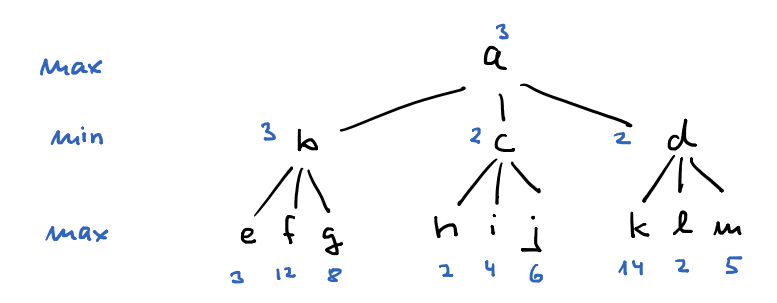
\includegraphics[height=4cm]{\pfad/Spielbaum/Aufgaben/minmax_01/minmax_01.png}
\begin{lstlisting}
b. Reihenfolge des Knotenbesuchs: b:3 c:2 d:2 a:3
c. Bester Zug: b
d. Reihenfolge des Blattbesuchs: e f g h # k l #
\end{lstlisting}
\end{solutionbox}
